%% Mikiri, short version in the IJCAI format (anonymous submission).
%% Built with the IJCAI-ECAI 2026 author kit; swap in the 2027 kit when it is released.
\documentclass{article}
\pdfpagewidth=8.5in
\pdfpageheight=11in

\usepackage{ijcai26}
\usepackage{iftex}
\ifPDFTeX
  \usepackage{times}
\else
  % XeTeX and LuaTeX have no Type 1 Times; TeX Gyre Termes is the metric-compatible OpenType face.
  \usepackage{fontspec}
  \setmainfont{texgyretermes}[Extension=.otf, UprightFont=*-regular, BoldFont=*-bold,
    ItalicFont=*-italic, BoldItalicFont=*-bolditalic, Ligatures=TeX]
\fi
\usepackage{url}
\usepackage[hidelinks]{hyperref}
\usepackage[utf8]{inputenc}
\usepackage[small]{caption}
\usepackage{graphicx}
\usepackage{amsmath}
\usepackage{amssymb}
\usepackage{booktabs}
\usepackage[switch]{lineno}
\linenumbers
\urlstyle{same}
\graphicspath{{../../results/figures/}}

% Generated by experiments/paper_tables.py. Do not edit.
\newcommand{\mainGames}{\textbf{??}}
\newcommand{\mainRecord}{\textbf{??}}
\newcommand{\mainScore}{\textbf{??}}
\newcommand{\mainElo}{\textbf{??}}
\newcommand{\mainEloLo}{\textbf{??}}
\newcommand{\mainEloHi}{\textbf{??}}
\newcommand{\mainVisits}{\textbf{??}}
\newcommand{\mainRestart}{\textbf{??}}
\newcommand{\mainEvals}{\textbf{??}}
\newcommand{\mainBaseEvals}{\textbf{??}}
\newcommand{\mainHitRate}{\textbf{??}}
\newcommand{\mainHitLate}{\textbf{??}}
\newcommand{\mainMemory}{\textbf{??}}
\newcommand{\strictGames}{\textbf{??}}
\newcommand{\strictRecord}{\textbf{??}}
\newcommand{\strictScore}{\textbf{??}}
\newcommand{\strictElo}{\textbf{??}}
\newcommand{\strictEloLo}{\textbf{??}}
\newcommand{\strictEloHi}{\textbf{??}}
\newcommand{\strictVisits}{\textbf{??}}
\newcommand{\strictRestart}{\textbf{??}}
\newcommand{\strictEvals}{\textbf{??}}
\newcommand{\strictBaseEvals}{\textbf{??}}
\newcommand{\strictHitRate}{\textbf{??}}
\newcommand{\strictHitLate}{\textbf{??}}
\newcommand{\strictMemory}{\textbf{??}}
\newcommand{\pairedGames}{\textbf{??}}
\newcommand{\pairedRecord}{\textbf{??}}
\newcommand{\pairedScore}{\textbf{??}}
\newcommand{\pairedElo}{\textbf{??}}
\newcommand{\pairedEloLo}{\textbf{??}}
\newcommand{\pairedEloHi}{\textbf{??}}
\newcommand{\pairedVisits}{\textbf{??}}
\newcommand{\pairedRestart}{\textbf{??}}
\newcommand{\pairedEvals}{\textbf{??}}
\newcommand{\pairedBaseEvals}{\textbf{??}}
\newcommand{\pairedHitRate}{\textbf{??}}
\newcommand{\pairedHitLate}{\textbf{??}}
\newcommand{\pairedMemory}{\textbf{??}}
\newcommand{\memonlyGames}{\textbf{??}}
\newcommand{\memonlyRecord}{\textbf{??}}
\newcommand{\memonlyScore}{\textbf{??}}
\newcommand{\memonlyElo}{\textbf{??}}
\newcommand{\memonlyEloLo}{\textbf{??}}
\newcommand{\memonlyEloHi}{\textbf{??}}
\newcommand{\memonlyVisits}{\textbf{??}}
\newcommand{\memonlyRestart}{\textbf{??}}
\newcommand{\memonlyEvals}{\textbf{??}}
\newcommand{\memonlyBaseEvals}{\textbf{??}}
\newcommand{\memonlyHitRate}{\textbf{??}}
\newcommand{\memonlyHitLate}{\textbf{??}}
\newcommand{\memonlyMemory}{\textbf{??}}
\newcommand{\fullGames}{\textbf{??}}
\newcommand{\fullRecord}{\textbf{??}}
\newcommand{\fullScore}{\textbf{??}}
\newcommand{\fullElo}{\textbf{??}}
\newcommand{\fullEloLo}{\textbf{??}}
\newcommand{\fullEloHi}{\textbf{??}}
\newcommand{\fullVisits}{\textbf{??}}
\newcommand{\fullRestart}{\textbf{??}}
\newcommand{\fullEvals}{\textbf{??}}
\newcommand{\fullBaseEvals}{\textbf{??}}
\newcommand{\fullHitRate}{\textbf{??}}
\newcommand{\fullHitLate}{\textbf{??}}
\newcommand{\fullMemory}{\textbf{??}}
\newcommand{\longGames}{\textbf{??}}
\newcommand{\longRecord}{\textbf{??}}
\newcommand{\longScore}{\textbf{??}}
\newcommand{\longElo}{\textbf{??}}
\newcommand{\longEloLo}{\textbf{??}}
\newcommand{\longEloHi}{\textbf{??}}
\newcommand{\longVisits}{\textbf{??}}
\newcommand{\longRestart}{\textbf{??}}
\newcommand{\longEvals}{\textbf{??}}
\newcommand{\longBaseEvals}{\textbf{??}}
\newcommand{\longHitRate}{\textbf{??}}
\newcommand{\longHitLate}{\textbf{??}}
\newcommand{\longMemory}{\textbf{??}}
\newcommand{\bhundredGames}{\textbf{??}}
\newcommand{\bhundredRecord}{\textbf{??}}
\newcommand{\bhundredScore}{\textbf{??}}
\newcommand{\bhundredElo}{\textbf{??}}
\newcommand{\bhundredEloLo}{\textbf{??}}
\newcommand{\bhundredEloHi}{\textbf{??}}
\newcommand{\bhundredVisits}{\textbf{??}}
\newcommand{\bhundredRestart}{\textbf{??}}
\newcommand{\bhundredEvals}{\textbf{??}}
\newcommand{\bhundredBaseEvals}{\textbf{??}}
\newcommand{\bhundredHitRate}{\textbf{??}}
\newcommand{\bhundredHitLate}{\textbf{??}}
\newcommand{\bhundredMemory}{\textbf{??}}
\newcommand{\bfourGames}{\textbf{??}}
\newcommand{\bfourRecord}{\textbf{??}}
\newcommand{\bfourScore}{\textbf{??}}
\newcommand{\bfourElo}{\textbf{??}}
\newcommand{\bfourEloLo}{\textbf{??}}
\newcommand{\bfourEloHi}{\textbf{??}}
\newcommand{\bfourVisits}{\textbf{??}}
\newcommand{\bfourRestart}{\textbf{??}}
\newcommand{\bfourEvals}{\textbf{??}}
\newcommand{\bfourBaseEvals}{\textbf{??}}
\newcommand{\bfourHitRate}{\textbf{??}}
\newcommand{\bfourHitLate}{\textbf{??}}
\newcommand{\bfourMemory}{\textbf{??}}
\newcommand{\beightGames}{\textbf{??}}
\newcommand{\beightRecord}{\textbf{??}}
\newcommand{\beightScore}{\textbf{??}}
\newcommand{\beightElo}{\textbf{??}}
\newcommand{\beightEloLo}{\textbf{??}}
\newcommand{\beightEloHi}{\textbf{??}}
\newcommand{\beightVisits}{\textbf{??}}
\newcommand{\beightRestart}{\textbf{??}}
\newcommand{\beightEvals}{\textbf{??}}
\newcommand{\beightBaseEvals}{\textbf{??}}
\newcommand{\beightHitRate}{\textbf{??}}
\newcommand{\beightHitLate}{\textbf{??}}
\newcommand{\beightMemory}{\textbf{??}}
\newcommand{\bignetGames}{\textbf{??}}
\newcommand{\bignetRecord}{\textbf{??}}
\newcommand{\bignetScore}{\textbf{??}}
\newcommand{\bignetElo}{\textbf{??}}
\newcommand{\bignetEloLo}{\textbf{??}}
\newcommand{\bignetEloHi}{\textbf{??}}
\newcommand{\bignetVisits}{\textbf{??}}
\newcommand{\bignetRestart}{\textbf{??}}
\newcommand{\bignetEvals}{\textbf{??}}
\newcommand{\bignetBaseEvals}{\textbf{??}}
\newcommand{\bignetHitRate}{\textbf{??}}
\newcommand{\bignetHitLate}{\textbf{??}}
\newcommand{\bignetMemory}{\textbf{??}}
\newcommand{\thirteenGames}{\textbf{??}}
\newcommand{\thirteenRecord}{\textbf{??}}
\newcommand{\thirteenScore}{\textbf{??}}
\newcommand{\thirteenElo}{\textbf{??}}
\newcommand{\thirteenEloLo}{\textbf{??}}
\newcommand{\thirteenEloHi}{\textbf{??}}
\newcommand{\thirteenVisits}{\textbf{??}}
\newcommand{\thirteenRestart}{\textbf{??}}
\newcommand{\thirteenEvals}{\textbf{??}}
\newcommand{\thirteenBaseEvals}{\textbf{??}}
\newcommand{\thirteenHitRate}{\textbf{??}}
\newcommand{\thirteenHitLate}{\textbf{??}}
\newcommand{\thirteenMemory}{\textbf{??}}
\newcommand{\nineGames}{\textbf{??}}
\newcommand{\nineRecord}{\textbf{??}}
\newcommand{\nineScore}{\textbf{??}}
\newcommand{\nineElo}{\textbf{??}}
\newcommand{\nineEloLo}{\textbf{??}}
\newcommand{\nineEloHi}{\textbf{??}}
\newcommand{\nineVisits}{\textbf{??}}
\newcommand{\nineRestart}{\textbf{??}}
\newcommand{\nineEvals}{\textbf{??}}
\newcommand{\nineBaseEvals}{\textbf{??}}
\newcommand{\nineHitRate}{\textbf{??}}
\newcommand{\nineHitLate}{\textbf{??}}
\newcommand{\nineMemory}{\textbf{??}}
\newcommand{\unihalfGames}{400}
\newcommand{\unihalfRecord}{77--301--22}
\newcommand{\unihalfScore}{22.0}
\newcommand{\unihalfElo}{-220}
\newcommand{\unihalfEloLo}{-262}
\newcommand{\unihalfEloHi}{-181}
\newcommand{\unihalfVisits}{100}
\newcommand{\unihalfRestart}{100}
\newcommand{\unihalfEvals}{40}
\newcommand{\unihalfBaseEvals}{71}
\newcommand{\unihalfHitRate}{0.0}
\newcommand{\unihalfHitLate}{\textbf{??}}
\newcommand{\unihalfMemory}{0}
\newcommand{\unisameGames}{400}
\newcommand{\unisameRecord}{185--183--32}
\newcommand{\unisameScore}{50.2}
\newcommand{\unisameElo}{+2}
\newcommand{\unisameEloLo}{-30}
\newcommand{\unisameEloHi}{+35}
\newcommand{\unisameVisits}{200}
\newcommand{\unisameRestart}{200}
\newcommand{\unisameEvals}{76}
\newcommand{\unisameBaseEvals}{76}
\newcommand{\unisameHitRate}{0.0}
\newcommand{\unisameHitLate}{\textbf{??}}
\newcommand{\unisameMemory}{0}
\newcommand{\unirootGames}{400}
\newcommand{\unirootRecord}{247--126--27}
\newcommand{\unirootScore}{65.1}
\newcommand{\unirootElo}{+108}
\newcommand{\unirootEloLo}{+76}
\newcommand{\unirootEloHi}{+143}
\newcommand{\unirootVisits}{283}
\newcommand{\unirootRestart}{283}
\newcommand{\unirootEvals}{98}
\newcommand{\unirootBaseEvals}{73}
\newcommand{\unirootHitRate}{0.0}
\newcommand{\unirootHitLate}{\textbf{??}}
\newcommand{\unirootMemory}{0}
\newcommand{\unidoubleGames}{400}
\newcommand{\unidoubleRecord}{310--73--17}
\newcommand{\unidoubleScore}{79.6}
\newcommand{\unidoubleElo}{+237}
\newcommand{\unidoubleEloLo}{+198}
\newcommand{\unidoubleEloHi}{+280}
\newcommand{\unidoubleVisits}{400}
\newcommand{\unidoubleRestart}{400}
\newcommand{\unidoubleEvals}{132}
\newcommand{\unidoubleBaseEvals}{73}
\newcommand{\unidoubleHitRate}{0.0}
\newcommand{\unidoubleHitLate}{\textbf{??}}
\newcommand{\unidoubleMemory}{0}
\newcommand{\pilotGames}{240}
\newcommand{\pilotRecord}{169--60--11}
\newcommand{\pilotScore}{72.7}
\newcommand{\pilotElo}{+170}
\newcommand{\pilotEloLo}{+125}
\newcommand{\pilotEloHi}{+219}
\newcommand{\pilotVisits}{201}
\newcommand{\pilotRestart}{252}
\newcommand{\pilotEvals}{96}
\newcommand{\pilotBaseEvals}{77}
\newcommand{\pilotHitRate}{0.0}
\newcommand{\pilotHitLate}{\textbf{??}}
\newcommand{\pilotMemory}{0}

% paired differences
\newcommand{\pairedVmctsTwo}{0.54 [0.28, 0.84]}
\newcommand{\pairedVmctsFour}{0.35 [0.09, 0.65]}
\newcommand{\pairedDsTwo}{0.65 [0.40, 0.93]}
\newcommand{\pairedDsRateFour}{0.03 [-0.16, 0.27]}


\title{Mikiri: Knowing When a Frozen Go Engine Has Searched Enough}

\author{
    Anonymous submission
}

\begin{document}
\maketitle

\begin{abstract}
A strong Go player glances at a forced recapture and plays it. The same player may sit for ten minutes over a fight that decides the game. Engines in the AlphaZero family do neither: they give every move the same search budget, and that is how they are compared. We ask how much that habit costs, and how much of it a frozen engine can recover with its network and its search left exactly as they are. Mikiri wraps KataGo and climbs a short ladder of search budgets, stopping at the first rung where the winrate still at stake no longer pays for the next rung. To build and test it we searched 6{,}000 positions at seven budgets and scored every candidate move with an independent search, which gives a yardstick that the engine cannot grade itself on. Offline, Mikiri matches uniform search at 1.8 to 2.1 times the visits, ahead of ten published stopping rules re-implemented on the same engine. In play against KataGo at the same visits it gains $\longElo$ Elo over \longGames{} games (95\% interval $\longEloLo$ to $\longEloHi$), and it draws level with KataGo given twice its visits. Doubling KataGo's own budget is worth $\unidoubleElo$, and the strongest prior rule, played the same way, gains $\vmctsElo$. One small idea does most of the work: divide the predicted stake by the price of the next rung. It turns stopping signals that are worse than no gate into gains, and it improves other people's rules too. We also report what did not work: similar positions do not share answers, and an exact memory of past searches saves visits but almost no network evaluations.
\end{abstract}

\section{Introduction}

Watch a strong player and you will see two kinds of move. Some are played almost before the opponent's stone has settled: a recapture, a connection, the only move. Others get long, visible thought. The player is not being inconsistent. They are spending attention where the game can still change.

Engines in the AlphaGo line \cite{silver2016mastering,silver2017mastering} do not make that distinction. They choose a move with a tree search guided by a policy network, which proposes moves, and a value network, which judges positions. The search is given a fixed number of \emph{visits}, which count how many times it descends the tree, and strength is measured by how well it plays at that number. KataGo \cite{wu2019accelerating}, the strongest engine anyone can download, follows the convention. At 200 visits per move, a forced recapture and a whole-board fight get 200 visits each.

How much does that cost? The question is older than neural engines. Time management for Monte-Carlo tree search was studied when the engines were weaker and the gains from thinking longer were larger \cite{huang2010time,baier2016time}. For AlphaZero-style agents, the evidence that a per-move budget helps comes from 9$\times$9 boards and small networks \cite{lan2021learning,ye2022spending,muppidi2026finding}, and KataGo already adapts its search inside the tree \cite{katago_methods}. It is reasonable to suspect that a modern engine on the full board has little left to gain. We did not know, and we found no measurement.

So we built one. Mikiri is a wrapper that changes nothing about KataGo except how many visits a move receives. It searches a position at 50 visits and asks a small model whether the decision is settled. If not, it searches at the next rung of a ladder, 200 visits, and asks again. The model predicts how much winrate the current choice might still be giving up, and the search stops when that stake, divided by the visits the next rung would cost, falls below a threshold. The name is a Japanese word for the judgment that one has seen enough.

Measuring this properly turned out to be most of the work, because a search cannot grade its own choices. Our testbed scores every candidate move with a separate search that is forced to play it, counts compute three ways, and plays both sides with the same engine and network. Along the way we tested the idea this project started from, retrieving analyses of similar positions, and found that it does not help a frozen engine. We report that too.

In summary, this paper contributes:
\begin{enumerate}
\item \textbf{A testbed with exact accounting.} Both players use the same engine, network and move-selection rule. Compute is reported as visits, as visits with every restarted search charged, and as network evaluations counted per player (Section~\ref{sec:testbed}).
\item \textbf{A ladder dataset with independent labels.} 6{,}000 positions searched at seven budgets, every chosen move scored by a forced search. It shows where search error lives, and it predicts match results before the games are played (Sections~\ref{sec:ladder} and~\ref{sec:matches}).
\item \textbf{A stopping rule worth nearly a doubling of search.} $\longElo$ Elo over KataGo at equal visits, a draw against KataGo at twice the visits, and $\strictElo$ Elo with 20\% fewer (Section~\ref{sec:matches}).
\item \textbf{A comparison with ten published rules} on one engine, offline for all of them and in play for the two strongest (Sections~\ref{sec:baselines} and~\ref{sec:matches}).
\item \textbf{The rate rule.} Pricing the next rung matters more than the model that predicts the stake, and it improves prior rules as well (Section~\ref{sec:offline}).
\item \textbf{Two negative results} on what a frozen engine can retrieve (Section~\ref{sec:retrieval}).
\end{enumerate}

\section{Related Work}

\textbf{Deciding how long to search.} Huang \textit{et al.}~\shortcite{huang2010time} extend a search when the most-visited move is not the one with the highest value, a sign that the search has not made up its mind. Baier and Winands~\shortcite{baier2016time} compare several such strategies across five games and find that stopping early, once the leader can no longer be overtaken, is the most reliable; Leela Chess Zero ships a version of that rule together with a stop on how much the visit distribution is still changing \cite{lc0_options}. Hay \textit{et al.}~\shortcite{hay2012selecting} and Kaufmann and Koolen~\shortcite{kaufmann2017monte} derive stopping rules from the value of information and from best-arm identification. For AlphaZero-style agents, DS-MCTS \cite{lan2021learning} trains networks to predict whether the current choice will survive more search, V-MCTS \cite{ye2022spending} stops when virtually expanded visit distributions have converged, and Muppidi \textit{et al.}~\shortcite{muppidi2026finding} choose a budget before the search starts. These neural results come from 9$\times$9 boards or small planners. We re-implement all of them on 19$\times$19 with a strong network and test them side by side (Section~\ref{sec:baselines}).

\textbf{Reusing search.} Transposition tables and graph search share statistics between identical positions inside one search \cite{childs2008transpositions,czech2021improving}, and opening books do so across games \cite{katagobooks}. Retrieving similar positions helps agents whose networks are trained to read their neighbours \cite{humphreys2022retrieval,goyal2022retrieval}, and memory can help inside a single search \cite{xiao2018memory}. Our question is narrower: what can an engine reuse when its network is fixed?

\section{Testbed}
\label{sec:testbed}

Every number in this paper comes from one harness, built so that the two players differ only in how they spend visits.

\textbf{Engine and rules.} Both players query KataGo v1.18.2 through its analysis engine. Each query is a fresh search with an exact visit limit and one search thread, so no player inherits a tree from an earlier move and a visit means the same thing at every budget. The network is the 18-block \texttt{b18c384nbt} unless stated. Games use area scoring, positional superko and komi 7, the value at which the engine rates the empty board as even. Both players pick moves the way KataGo does by default, sampling in proportion to visits$^{1/T}$ with a temperature $T$ that decays from 0.5 to 0.1 over the game. A player resigns after three consecutive turns below 3\% winrate.

\textbf{Three ways to count compute.} This needs care, because Mikiri restarts its search. A position searched at 50 visits and then at 200 has been asked for 250 visits of work; whether it has done 250 visits of work depends on the engine. With one thread and cached network evaluations the 50-visit tree is a prefix of the 200-visit tree, and we measured this: on fresh engines, a 200-visit search followed by a 400-visit search evaluated 366 to 396 network rows, against 353 to 395 for the 400-visit search alone. We nonetheless report three numbers for every match and let the reader choose: \emph{visits}, the size of the deepest search per move, which is what an in-engine implementation would pay; \emph{restart visits}, the sum of every search requested, an upper bound; and \emph{evaluations}, the network rows each player's own engine process actually executed, read from its log. Budgets are matched on visits.

\textbf{Matches.} A match is a series of games from the empty board with alternating colours. Confidence intervals are bootstrap percentiles over colour-balanced pairs of games, and Elo is $-400\log_{10}(1/s-1)$ for a score $s$. As a check on the harness, KataGo against itself at 200 visits scores \unisameScore\% over \unisameGames{} games ($\unisameElo$ Elo).

\section{The Ladder Dataset}
\label{sec:ladder}

Before building a stopping rule we wanted to know what one could gain, position by position. We played 300 self-play games at budgets drawn log-uniformly from 30 to 200 visits and sampled 20 positions per game, which gives 6{,}000 positions from the distribution a low-budget player actually meets. Each position is searched at 50, 100, 200, 400, 800, 1{,}600 and 3{,}200 visits.

Here it gets a little tricky. The value a search reports for its own choice is exactly the estimate that might be wrong, so it cannot be the yardstick. Instead, for every distinct move that any rung chose, we run a separate 1{,}600-visit search restricted to that move at the root. Its winrate $q(s,a)$ is our value for playing $a$ in position $s$. Every move is scored the same way, by a search that did not choose it. The \emph{regret} of stopping at rung $k$ is $r_k(s)=\max_{a} q(s,a)-q(s,a_k(s))$, where $a_k$ is the move chosen at rung $k$ and the maximum runs over scored moves. Regret is in winrate, so it is small in positions that are already decided and large where the game can still turn, which is the behaviour we want from a stake.

To compare policies we convert regret back into visits. For a policy with mean regret $\bar r$ we find the uniform budget with the same mean regret, interpolating the uniform curve in log visits, and divide it by the policy's own mean cost. We call this ratio the \emph{compute multiplier}: how many times more visits uniform search needs to do as well.

\textbf{Regret is rare and concentrated.} At 200 visits the engine gives up 0.99\% of winrate per move on average. That average hides the shape. 71\% of positions carry no regret at all, and the worst tenth hold 84\% of the total (Figure~\ref{fig:anatomy}). Regret also depends on where in the game you are: 0.19\% per move over the first 40 moves and 1.4 to 1.6\% after move 100. A stopping rule that knew the true regret, and stopped at the first rung with none, would match uniform search at twelve times the visits for a 200-visit budget. That is the room available.

\begin{figure}[t]
\centering
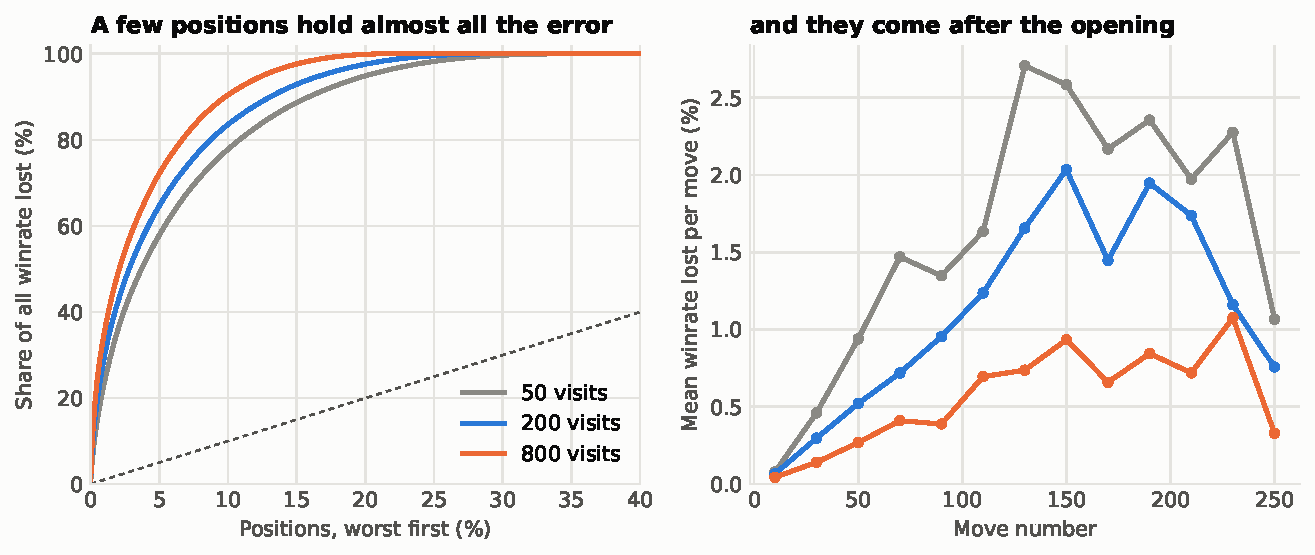
\includegraphics[width=\linewidth]{regret_anatomy}
\caption{Left: share of all regret held by the worst positions, at three budgets. Right: mean regret by move number.}
\label{fig:anatomy}
\end{figure}

Figure~\ref{fig:case} shows what one of the costly positions looks like. At 50 and at 200 visits the engine chooses a move that an independent search rates at 11\%. At 800 visits it finds one rated at 62\%. The game turns on whether the search is allowed to continue.

\begin{figure}[t]
\centering
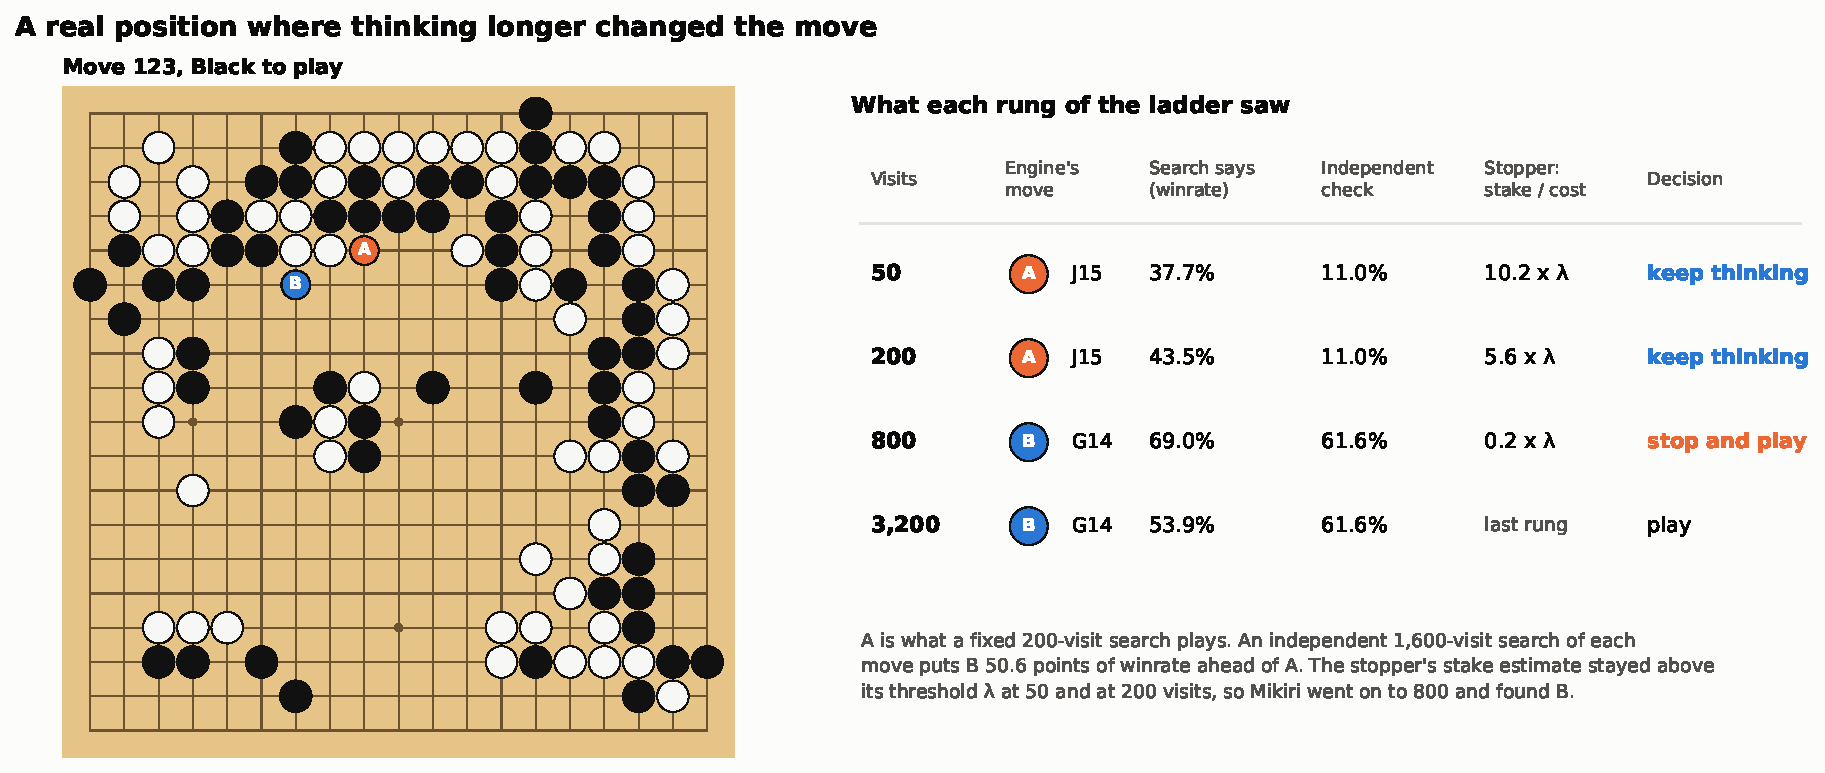
\includegraphics[width=\linewidth]{case_study}
\caption{A position where the stopper keeps searching and the move changes. The threshold $\lambda$ shown gives a mean cost of 200 visits.}
\label{fig:case}
\end{figure}

\textbf{No single signal finds it.} The natural first attempt is to read one statistic off the search. Table~\ref{tab:auc} asks how well each one ranks positions by whether more than 0.5\% of winrate is still on the table. Measures of how contested the root is, such as the top move's share of visits, reach an AUC of about 0.74. KataGo's own prediction of its short-term winrate error, which it uses inside the tree, reaches only 0.58 to 0.60 as a predictor of whether the root decision will improve. The classical cue, that the most-visited move is not the highest-valued one \cite{huang2010time}, reaches 0.59 to 0.61. The reason is plain once you look at the positions: contested roots are common, and most are contested between moves of nearly equal value, where being wrong costs nothing.

\begin{table}[t]
\centering\small
\begin{tabular}{lrrr}
\toprule
Signal & 50 & 200 & 800 \\
\midrule
Top move's visit share & 0.75 & 0.74 & 0.74 \\
LCB margin & 0.74 & 0.73 & 0.73 \\
v1 entropy gate & 0.73 & 0.73 & 0.74 \\
KL(visits, prior) & 0.65 & 0.63 & 0.61 \\
Most-visited is not best-valued & 0.60 & 0.59 & 0.61 \\
KataGo's predicted winrate error & 0.58 & 0.58 & 0.60 \\
Searched minus raw winrate & 0.57 & 0.56 & 0.56 \\
\bottomrule
\end{tabular}

\caption{AUC for ranking positions by remaining regret above 0.5\%, from the search at 50, 200 and 800 visits.}
\label{tab:auc}
\end{table}

\section{Mikiri}

Figure~\ref{fig:pipeline} shows how Mikiri decides one move. The parts are a ladder of budgets, a model that predicts the stake, a rule that prices it, a ledger that keeps the total honest, and a memory.

\begin{figure*}[t]
\centering
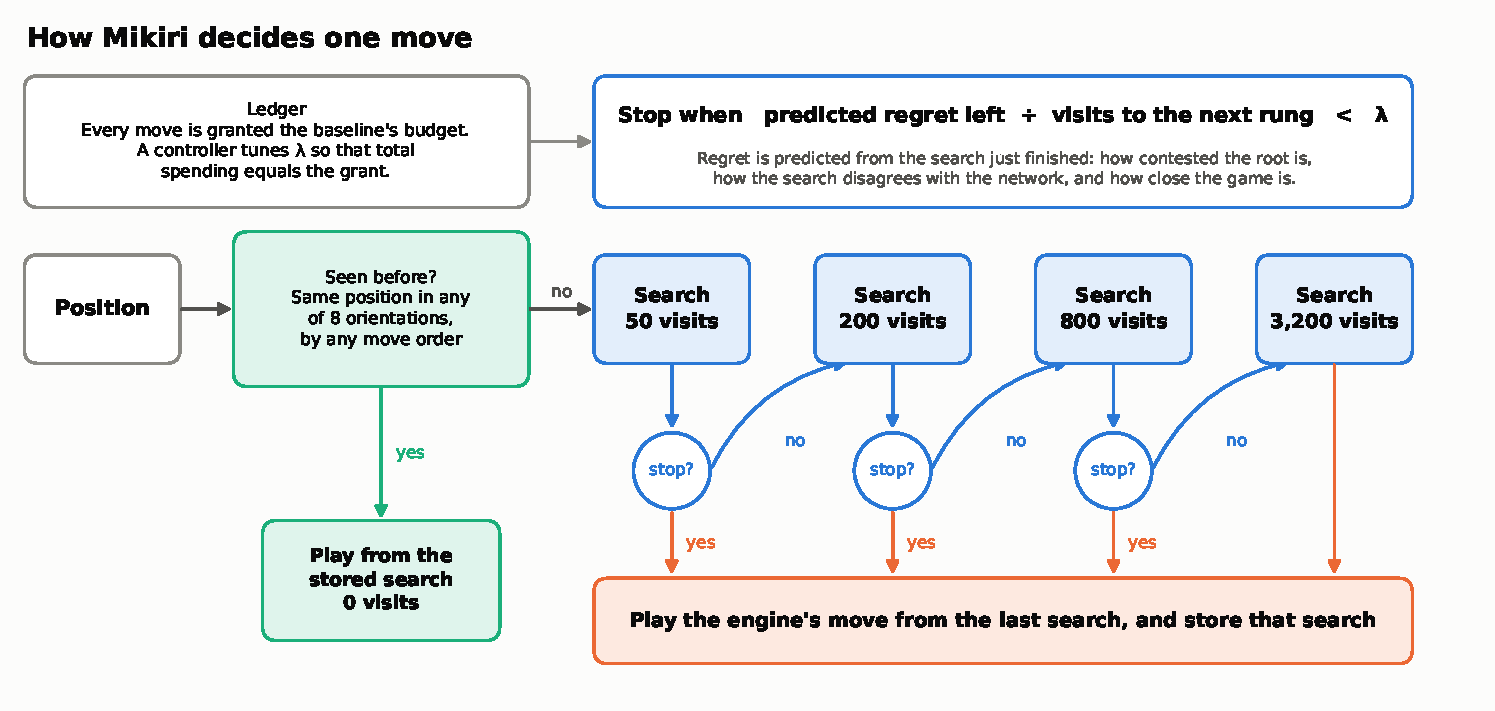
\includegraphics[width=0.86\textwidth]{pipeline}
\caption{How Mikiri decides one move.}
\label{fig:pipeline}
\end{figure*}

\textbf{The rate rule.} Consider what the stopping decision is actually trading. Let the ladder have rungs $v_1<\dots<v_m$, and let a stopping policy $\pi$ stop position $s$ at rung $\pi(s)$. We want the policy that gives up the least winrate for a fixed average cost,
\begin{equation}
  \min_\pi \; \mathbb{E}\bigl[r_{\pi(s)}(s)\bigr] \quad \text{s.t.} \quad \mathbb{E}\bigl[v_{\pi(s)}\bigr] \le B .
\end{equation}
Put a multiplier $\lambda$ on the constraint and the problem falls apart into one decision per position: each minimises $r_k(s)+\lambda v_k$. At rung $j$ the visits already spent are gone, so continuing one more rung is worth it exactly when $\mathbb{E}[r_j-r_{j+1}\mid x] > \lambda\,(v_{j+1}-v_j)$, where $x$ is whatever the finished search shows. The reduction $r_j-r_{j+1}$ can be at most $r_j$. Replace it by a prediction $\hat r_j(x)$ of the regret remaining, and the rule becomes: stop when
\begin{equation}
  \frac{\hat r_j(x)}{v_{j+1}-v_j} < \lambda .
  \label{eq:rate}
\end{equation}
One $\lambda$ prices every decision on the ladder alike. On a geometric ladder the next rung costs more each time, so going from 800 to 3{,}200 visits needs four times the stake that going from 200 to 800 does. A flat threshold on $\hat r_j$ ignores that price and, as we will see, spends most of a long ladder's budget on a handful of positions that no amount of search resolves.

\textbf{The model.} $\hat r$ is a gradient-boosted ensemble of 150 trees of depth 3, fitted to the square root of regret with all non-final rungs pooled. Its 30 inputs come from the search that just finished, at no extra engine cost: how contested the root is (visit shares, entropy, the margin between the best move's lower confidence bound and its nearest rival), how the search disagrees with the network (priors, the KL divergence from prior to visits, raw against searched winrate), what is at stake (winrate, its distance from 50\%, score), KataGo's own raw predictions of its error, the game phase, and what changed since the previous rung. Every offline number we report is cross-fitted by game, so no position is scored by a model that saw its game.

\textbf{The ledger.} Mikiri is granted the baseline's budget $B$ for every move, and a ledger records what it spends. The offline frontier gives a map $\lambda(c)$ from a target mean cost $c$ to a threshold. After each move the controller sets the next target to $B$ plus the ledger's balance spread over a horizon of 3{,}000 moves, and divides by a running ratio of realised to commanded spending, which corrects for the difference between the dataset and real games. Spending tracks the grant to within 1\% in every match we report.

\textbf{Memory.} Finished searches from the first 80 moves are stored under a key that is invariant to the eight board symmetries and to move order. When a later game reaches the same position, Mikiri plays from the stored search and spends nothing.

\section{Offline Results}
\label{sec:offline}

\begin{figure}[t]
\centering
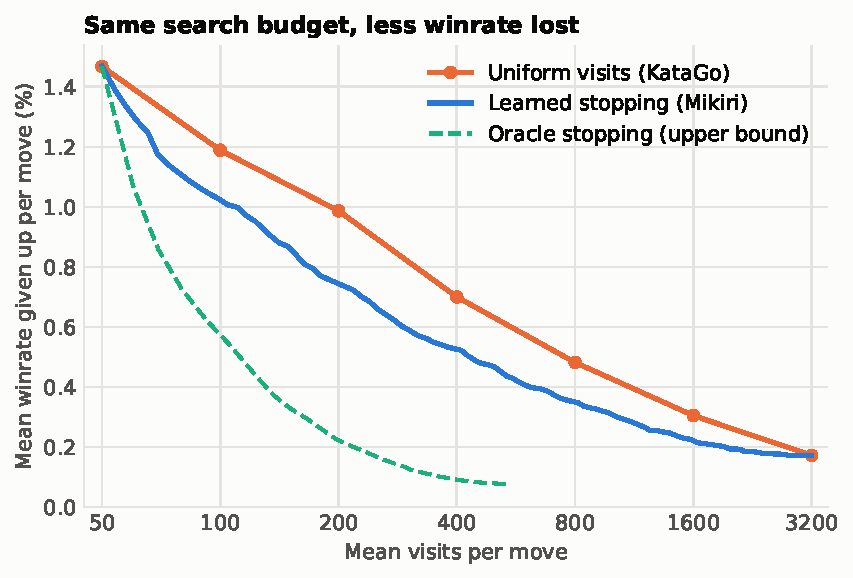
\includegraphics[width=0.95\linewidth]{frontier}
\caption{Mean regret against mean visits on the four-rung ladder, for uniform search, the learned stopper, and an oracle that knows the true regret.}
\label{fig:frontier}
\end{figure}

\textbf{Multiplier.} On the four-rung ladder (50, 200, 800, 3{,}200) the stopper at a mean cost of 200 visits gives up as little winrate as uniform search at 358, a multiplier of 1.80, and it stays between 1.69 and 1.88 for budgets from 100 to 800 visits (Figure~\ref{fig:frontier}). If every restarted search is charged in full, so that reaching the 800 rung costs $50+200+800$, the multiplier is 1.29 to 1.51. On the full doubling ladder it reaches 2.13.

\textbf{What matters, and what does not.} Removing the features that track change between rungs, removing KataGo's raw error predictions, or keeping only seven features changes the multiplier at 200 visits by at most 0.09. Three hundred labeled positions already give 1.50. Two choices do matter. Fitting the square root of regret rather than regret raises the multiplier from 1.74 to 1.82, because a few very large blunders otherwise dominate the fit. Replacing the rate rule with a flat threshold lowers it to 1.41. Figure~\ref{fig:rate} shows the same contrast for hand-written signals: with a flat threshold, the entropy gate of an earlier prototype is worse than no gate at all (0.63), and with the rate rule the same signal is a gain (1.16).

\begin{figure}[t]
\centering
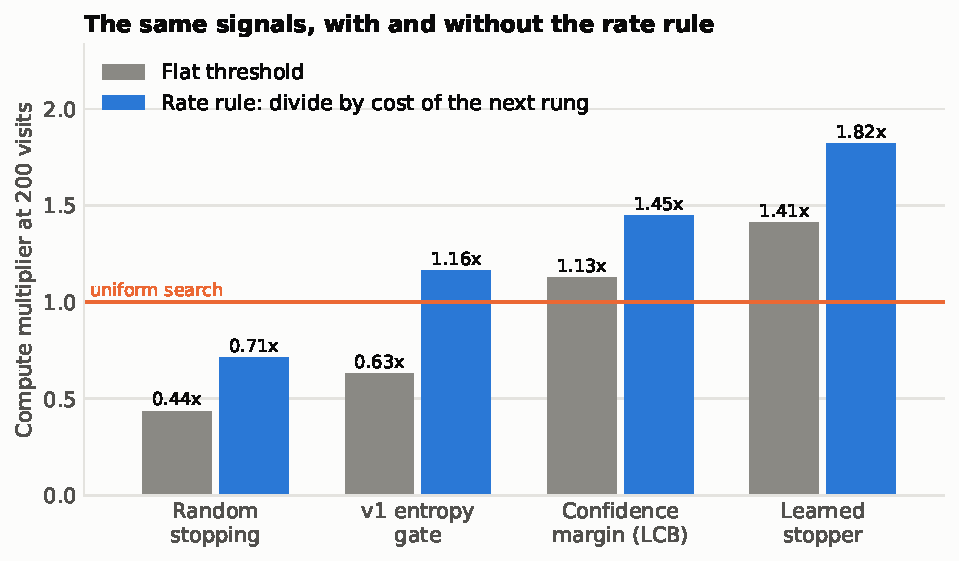
\includegraphics[width=0.92\linewidth]{rate_rule}
\caption{Four stopping signals on the four-rung ladder at 200 visits, with a flat threshold and with the rate rule.}
\label{fig:rate}
\end{figure}

\subsection{Comparison with Prior Rules}
\label{sec:baselines}

\begin{table*}[t]
\centering\small
\begin{tabular}{llll}
\toprule
Rule & As published, 200 & As published, 400 & With rate rule, 200 \\
\midrule
VOI stop \cite{hay2012selecting} & 0.34 [0.30, 0.40] & 0.24 [0.20, 0.31] & 1.05 [0.86, 1.21] \\
BAI stop \cite{kaufmann2017monte} & 0.77 [0.63, 1.01] & 0.59 [0.50, 0.71] & 1.18 [1.09, 1.29] \\
BEHIND \cite{huang2010time} & 0.89 at 174 & 0.89 at 348 & -- \\
STOP, $p=0.45$ \cite{baier2016time} & 1.25 at 134 & 1.19 at 512 & -- \\
Smart pruning \cite{lc0_options} & 1.17 at 159 & 1.21 at 308 & -- \\
CLOSE \cite{baier2016time} & 1.15 at 229 & 1.11 at 453 & -- \\
UNST \cite{huang2010time} & 1.21 at 239 & 1.17 at 475 & -- \\
KLD gain \cite{lc0_options} & 1.32 [1.18, 1.49] & 1.23 [1.02, 1.42] & -- \\
State only \cite{muppidi2026finding} & 1.18 [0.97, 1.40] & 1.02 [0.89, 1.23] & 1.54 [1.35, 1.74] \\
DS-MCTS \cite{lan2021learning} & 1.48 [1.28, 1.73] & 1.48 [1.29, 1.73] & 1.75 [1.60, 1.92] \\
V-MCTS \cite{ye2022spending} & 1.60 [1.44, 1.76] & 1.54 [1.36, 1.70] & -- \\
LCB margin & 1.14 [0.95, 1.36] & 0.82 [0.70, 0.97] & 1.45 [1.24, 1.70] \\
\textbf{Mikiri} & 1.40 [1.21, 1.63] & 1.35 [1.15, 1.61] & \textbf{2.13 [1.88, 2.41]} \\
\bottomrule
\end{tabular}

\caption{Compute multipliers on the doubling ladder (above 1 is better than uniform search), with 95\% bootstrap intervals over games. Threshold rules are swept and shown at their best point for each budget; rules without a threshold are shown at the configuration nearest the budget, with its cost in visits.}
\label{tab:baselines}
\end{table*}

How does this compare with what has been published? We re-implemented ten stopping rules from their papers and source code and ran them on the same data, where every rule sees the same root statistics and is scored by the same forced values (Table~\ref{tab:baselines}). \emph{BEHIND} and \emph{UNST} search longer when the player is losing or when the most-visited move is not the highest-valued one \cite{huang2010time}. \emph{STOP} ends a search once the runner-up cannot overtake the leader in the visits that remain, or in a fraction $p$ of them, and \emph{CLOSE} extends it when the top two moves are close \cite{baier2016time}. \emph{Smart pruning} is Leela Chess Zero's form of STOP, shipped with a stop on the per-visit KL gain of the visit distribution \cite{lc0_options}. The \emph{VOI} rule stops when a bound on the value of further samples falls below their cost \cite{hay2012selecting}, and the \emph{BAI} rule when the leader's confidence interval separates from every rival's \cite{kaufmann2017monte}. The \emph{state-only} rule predicts regret from what is known before any search, in the spirit of Muppidi \textit{et al.}~\shortcite{muppidi2026finding}. Two learned rules are adaptations, and we do not claim they reproduce the authors' systems: for DS-MCTS we train a classifier on root statistics to the authors' label $U(s,n)$, in place of their board-input networks, and for V-MCTS we run the authors' virtual expansion on KataGo's root priors, visits and winrates with their published $r=0.2$ and $\epsilon=0.1$. Every rule is charged continuation cost, which is what a rule inside the engine pays. A reader who prefers to charge Mikiri for every restart should compare its four-rung figure of 1.44 at 200 visits with the 1.60 of V-MCTS, which stops inside one search and has nothing to restart. The matches in Section~\ref{sec:matches} settle that question in network evaluations.

Three things stand out. First, the two rules with a statistical stopping guarantee are far worse than uniform search here (0.34 and 0.77 at 200 visits). They stop on confidence in the leading move, and confidence in the leader says little about whether the game is still in doubt. Second, V-MCTS is the strongest prior rule, at 1.60, and Mikiri exceeds it by \pairedVmctsTwo{} at 200 visits and \pairedVmctsFour{} at 400, as paired differences over the same resampled games. Third, the rate rule improves every signal it can be applied to. It lifts the DS-MCTS classifier from 1.48 to 1.75, and at 400 visits that combination ties Mikiri (\pairedDsRateFour). The price on the next rung matters more than which learned signal it is attached to.

\textbf{What to predict, and how to price it.} Remaining regret is an upper bound on what continuing can recover, so one might ask whether the model should predict something closer to the derivation. Table~\ref{tab:targets} tries the alternatives it names: the gain from the next rung, the gain from the whole ladder, and the best recovery per visit over any continuation, $\max_{k>j}(r_j-r_k)/(v_k-v_j)$. With perfect information that last index reproduces the hindsight optimum (14.11 against 14.16), so it is the right quantity in principle. Learned from search statistics it trails remaining regret under the rate rule (1.63 to 1.87 against 1.83 to 2.14). The next-rung gain is weakest on both counts: myopic as an oracle, because it stops whenever one more rung does not help even if two more would, and noisy as a target. Pricing remaining regret by the visits to the top of the ladder is worse than no price at all. The rate rule works because it pairs a target that search statistics can predict with the one cost that is known exactly.

\begin{table}[t]
\centering\footnotesize
\setlength{\tabcolsep}{3.5pt}
\begin{tabular}{llrrrr}
\toprule
 & & Oracle, & \multicolumn{3}{c}{Learned, 200 visits} \\
Scored & Divided by & 100 visits & 4 & 6 & 7 rungs \\
\midrule
$r_j$ & 1 (flat) & 5.99 & 1.41 & 1.56 & 1.51 \\
$r_j$ (rate rule) & $v_{j+1}-v_j$ & 8.69 & 1.83 & 1.98 & 2.14 \\
$r_j$ & $v_m-v_j$ & 5.86 & 1.35 & 1.50 & 1.39 \\
$r_j-r_{j+1}$ & $v_{j+1}-v_j$ & 4.96 & 1.50 & 1.54 & 1.44 \\
$r_j-r_m$ & $v_{j+1}-v_j$ & 9.07 & 1.79 & 1.98 & 2.04 \\
$\max_{k>j}\frac{r_j-r_k}{v_k-v_j}$ & built in & 14.11 & 1.63 & 1.87 & 1.77 \\
\midrule
\multicolumn{2}{l}{Hindsight optimum} & 14.16 & -- & -- & -- \\
\bottomrule
\end{tabular}

\caption{Multipliers for different quantities to score at rung $j$ and prices to divide them by ($m$ is the top rung). Oracle: true quantity, four-rung ladder, 100 visits. Learned: the same model fitted to each quantity, 200 visits, three ladders.}
\label{tab:targets}
\end{table}

\textbf{Do the prior rules see something we miss?} If the hand-derived statistics behind those rules carried information the 30 features lack, feeding them to the regressor should help. We added the KLD gain, the VOI bound, the BAI gap and the V-MCTS distance as extra inputs, one at a time and all together. The multiplier at 200 visits moved from 2.14 to between 2.07 and 2.17, and no paired difference was distinguishable from zero in the direction of a gain. The rules differ in what they do with the root statistics; the statistics themselves are used up.

\section{Matches}
\label{sec:matches}

\begin{table*}[t]
\centering\small
\begin{tabular}{lrrrrrr}
\toprule
Player (vs.\ KataGo at 200 visits) & Games & W--L--D & Elo (95\% interval) & Visits & Restart & Evals \\
\midrule
KataGo, 100 visits & 400 & 77--301--22 & $-220$ ($-262$, $-181$) & 100 & 100 & 40 : 71 \\
KataGo, 283 visits & 400 & 247--126--27 & $+108$ ($+76$, $+143$) & 283 & 283 & 98 : 73 \\
KataGo, 400 visits & 400 & 310--73--17 & $+237$ ($+198$, $+280$) & 400 & 400 & 132 : 73 \\
\midrule
Mikiri, seven-rung ladder & \multicolumn{6}{c}{(running)} \\
Mikiri, six-rung ladder & 1,000 & 750--175--75 & $+228$ ($+203$, $+254$) & 201 & 304 & 102 : 78 \\
Mikiri, four-rung ladder & 1,000 & 728--196--76 & $+206$ ($+181$, $+232$) & 200 & 251 & 99 : 74 \\
Mikiri, four-rung, 175-visit grant & \multicolumn{6}{c}{(running)} \\
Mikiri, four-rung, 160-visit grant & 1,000 & 586--325--89 & $+93$ ($+72$, $+114$) & 160 & 197 & 80 : 74 \\
Mikiri, four-rung, 140-visit grant & \multicolumn{6}{c}{(running)} \\
Mikiri, four-rung, no move sampling & 800 & 561--183--56 & $+178$ ($+153$, $+205$) & 200 & 250 & 115 : 96 \\
\midrule
V-MCTS rule (Ye et al.) & 600 & 395--173--32 & $+135$ ($+108$, $+164$) & 200 & 350 & 87 : 72 \\
Mikiri's rule on the V-MCTS ladder & 600 & 404--160--36 & $+150$ ($+121$, $+180$) & 200 & 350 & 92 : 74 \\
DS-MCTS-style rule (Lan et al.) & 600 & 395--157--48 & $+146$ ($+117$, $+176$) & 200 & 351 & 105 : 77 \\
LCB margin with rate rule, no learning & \multicolumn{6}{c}{(running)} \\
Entropy gate, flat threshold & \multicolumn{6}{c}{(running)} \\
\midrule
Memory only & 600 & 276--292--32 & $-9$ ($-37$, $+19$) & 158 & 158 & 69 : 69 \\
Mikiri four-rung + memory & 1,200 & 908--219--73 & $+227$ ($+204$, $+250$) & 201 & 255 & 109 : 76 \\
\bottomrule
\end{tabular}

\caption{Matches against KataGo at 200 visits per move, 19$\times$19, same network. \emph{Visits} is the mean size of the deepest search per move, \emph{Restart} charges every search requested, and \emph{Evals} is network evaluations per move for the player and for its opponent.}
\label{tab:matches}
\end{table*}

Offline numbers are only a forecast. Here is what happened when the games were played.

\textbf{Equal visits.} With the six-rung ladder (50, 200, 400, 800, 1{,}600, 3{,}200) Mikiri scores \longScore\% (\longRecord), a gain of $\longElo$ Elo ($\longEloLo$ to $\longEloHi$). With the four-rung ladder it gains $\mainElo$ ($\mainEloLo$ to $\mainEloHi$) over \mainGames{} games. For scale, KataGo given twice the visits gains $\unidoubleElo$ (Table~\ref{tab:matches}). We then played that comparison directly: Mikiri at 200 visits against KataGo at 400. The result is level, \halfRecord{} over \halfGames{} games ($\halfElo$ Elo, $\halfEloLo$ to $\halfEloHi$), with Mikiri running \halfEvals{} network evaluations per move to KataGo's \halfBaseEvals.

\textbf{Fewer visits, and the strictest count.} A fixed-budget engine finds much of its next tree already cached, and Mikiri's searches vary in size, so less carries over and it runs more evaluations per visit. We therefore also held it below the opponent. Granted 160 visits, Mikiri requests fewer visits than KataGo even with every restart charged (\strictRestart{} against 200) and still gains $\strictElo$ Elo ($\strictEloLo$ to $\strictEloHi$). Counting evaluations, the cleanest comparison is with KataGo at 283 visits, which runs \unirootEvals{} per move and gains $\unirootElo$; Mikiri's six-rung ladder runs \longEvals{} and gains $\longElo$. Figure~\ref{fig:elo} places every match against the uniform curve under all three counts.

\begin{figure*}[t]
\centering
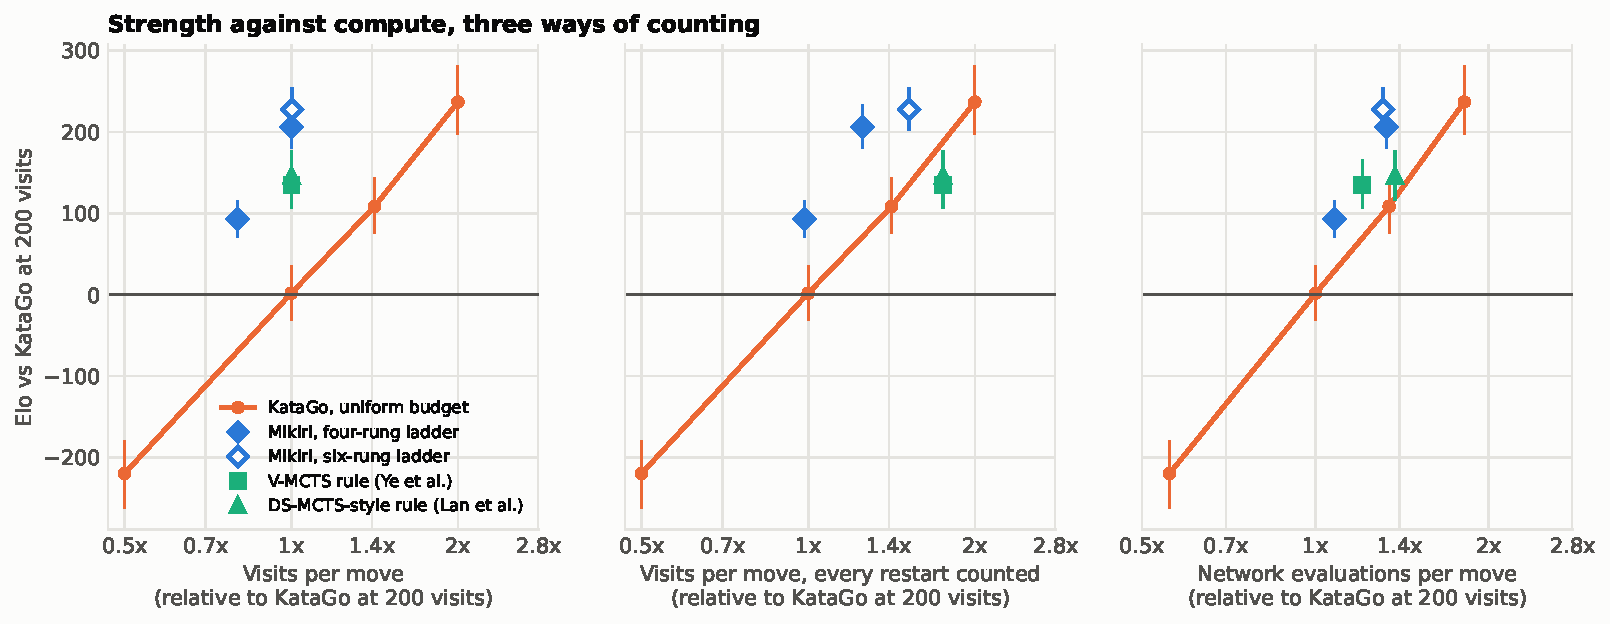
\includegraphics[width=0.9\textwidth]{elo_vs_compute}
\caption{Elo against KataGo at 200 visits as a function of compute relative to that baseline, counted three ways. The line is KataGo at uniform budgets; bars are 95\% intervals.}
\label{fig:elo}
\end{figure*}

\textbf{Is it the sampling?} A search that stops when one move dominates has sharper visit counts than a fixed-budget search, and KataGo samples among well-visited moves early in the game, so one could worry that Mikiri benefits from sampling rather than from better search. To rule that out we drew 400 balanced openings, played each twice with colours swapped, and had both players always play their top move. Mikiri gains $\pairedElo$ Elo ($\pairedEloLo$ to $\pairedEloHi$).

\textbf{Did the dataset predict this?} Take the cross-fitted regret at the cost Mikiri actually used, convert it to equivalent uniform visits, and read that budget's Elo off the measured uniform curve. This forecasts $+197$ for the four-rung match (measured $\mainElo$), $+126$ at 160 visits ($\strictElo$), $+225$ for the six-rung ladder ($\longElo$), $+145$ for the V-MCTS rule ($\vmctsElo$) and $+128$ for the DS-MCTS-style rule ($\dsmctsElo$). Each is within 35 Elo, and both prior rules are placed below Mikiri's equal-visit matches, as measured. The forecast has one clear miss: Mikiri's rule on the short V-MCTS ladder, forecast at $+196$ and measured at $\shortElo$ (Table~\ref{tab:forecast}). The ladder dataset is a useful guide for choosing among rules and no substitute for playing the games.

\begin{table}[t]
\centering\footnotesize
\setlength{\tabcolsep}{2pt}
\begin{tabular}{lrrrr}
\toprule
Rule & Visits & Equiv. & Forecast & Measured (95\% interval) \\
\midrule
Mikiri, four-rung & 160 & 297 & $+126$ & $+93$ ($+72$, $+114$) \\
Mikiri, four-rung & 200 & 360 & $+197$ & $+206$ ($+181$, $+232$) \\
Mikiri, six-rung & 201 & 387 & $+225$ & $+228$ ($+203$, $+254$) \\
V-MCTS rule & 200 & 312 & $+145$ & $+135$ ($+108$, $+164$) \\
\bottomrule
\end{tabular}

\caption{Elo forecast from the ladder dataset against Elo measured in play, versus KataGo at 200 visits.}
\label{tab:forecast}
\end{table}

\textbf{Prior rules in play.} We packaged the two strongest prior rules into the same player, under the same controller, at the same 200 visits. The V-MCTS rule gains $\vmctsElo$ Elo ($\vmctsEloLo$ to $\vmctsEloHi$) and the DS-MCTS-style classifier $\dsmctsElo$ ($\dsmctsEloLo$ to $\dsmctsEloHi$). The DS-MCTS-style rule runs \dsmctsEvals{} evaluations per move, more than Mikiri's six-rung ladder, so Mikiri is ahead of it however compute is counted. V-MCTS is the more interesting case. At equal visits Mikiri is ahead with intervals that do not overlap, but V-MCTS never searches past 400 visits, so more of its work is already in the cache: it runs \vmctsEvals{} evaluations per move to Mikiri's \mainEvals. Two more matches say what that means. Mikiri's stopper on V-MCTS's own ladder (50, 100, 200, 400), so that the rules differ in nothing else, gains $\shortElo$ ($\shortEloLo$ to $\shortEloHi$) at \shortEvals{} evaluations, which the match cannot separate from V-MCTS. Mikiri's four-rung ladder granted 175 visits, so that its evaluations match, gains $\midElo$ ($\midEloLo$ to $\midEloHi$) at \midEvals{} evaluations to V-MCTS's $\vmctsElo$ at \vmctsEvals: a lead of about 60 Elo whose intervals touch. So the lead at equal visits comes from ladders that reach 3{,}200 visits, which the rate rule makes affordable and V-MCTS does not exploit; those deep searches cost more evaluations per visit, and per evaluation the lead is smaller. For completeness, the LCB margin with the rate rule and no learning gains $\rulelcbElo$ ($\rulelcbEloLo$ to $\rulelcbEloHi$), and the entropy gate with a flat threshold $\vonegateElo$ ($\vonegateEloLo$ to $\vonegateEloHi$).

\textbf{Where the visits go.} Nobody told Mikiri when to think. It uses a third of the budget over the first 20 moves, where the dataset found almost no regret to recover, and about 270 visits per move around move 140. After move 60 it spends about 130 visits when it rates its winrate above 90\% and up to 330 when it is behind but not lost. It scores 76.2\% as Black and 77.0\% as White. All of this follows from predicting regret in winrate units, and none of it was programmed.

\textbf{Other settings.} The same model, trained once and never retrained, was played in further settings (Table~\ref{tab:other}).

\begin{table}[t]
\centering\footnotesize
\setlength{\tabcolsep}{3pt}
\begin{tabular}{lrrrr}
\toprule
Opponent and setting & Games & W--L--D & Elo (95\% interval) & Visits \\
\midrule
KataGo 100 visits, 19x19, b18 & 400 & 262--119--19 & $+130$ ($+95$, $+167$) & 100 \\
KataGo 400 visits, 19x19, b18 & \multicolumn{4}{c}{(running)} \\
KataGo 800 visits, 19x19, b18 & \multicolumn{4}{c}{(running)} \\
KataGo 200 visits, 19x19, b28 network & \multicolumn{4}{c}{(running)} \\
KataGo 200 visits, 13x13, b18 & \multicolumn{4}{c}{(running)} \\
KataGo 200 visits, 9x9, b18 & \multicolumn{4}{c}{(running)} \\
\bottomrule
\end{tabular}

\caption{The four-rung stopper, trained once on 19$\times$19 b18 positions, against KataGo at matched visits in other settings.}
\label{tab:other}
\end{table}

\section{What a Frozen Engine Can Retrieve}
\label{sec:retrieval}

This project began with a different idea: store deep analyses, find similar positions with a nearest-neighbour index, and reuse what was found. We tested it, and we tested the honest version of it.

\textbf{Exact memory.} Positions recur more than one might guess. Across 300 self-play games, a position at move 20 had occurred in an earlier game, up to symmetry, half of the time. In play, memory alone served \memonlyHitRate\% of moves over \memonlyGames{} games at \memonlyVisits{} visits per move, with strength unchanged ($\memonlyElo$ Elo, $\memonlyEloLo$ to $\memonlyEloHi$), which is what should happen when a hit returns the search that would have been run. It did not reduce network evaluations (\memonlyEvals{} per move against \memonlyBaseEvals). KataGo caches evaluations for the life of its process, so the positions that memory serves were already cheap.

\textbf{Approximate retrieval.} We embed positions with the raw policy and ownership maps, align over the eight symmetries, and offer the nearest stored position's 3{,}200-visit move as a proposal. Where the 200-visit and 3{,}200-visit moves differ (1{,}605 positions), the nearest neighbour's move is right 5.5\% of the time. The policy network's own best alternative is right 43\% of the time. A neighbour's move matches in 96\% of cases at similarity above 0.999, which in practice means the same position, and in 27\% at similarity between 0.90 and 0.97. Neighbours' regret predicts a position's regret with an AUC of 0.55. Go is unforgiving here: a stone's difference changes the answer, so proximity in a smooth embedding is weak evidence about the best move.

\section{Limitations}

Our results are for KataGo networks at 100 to 800 visits, against KataGo, a range where a doubling of visits is worth about 230 Elo. At tournament budgets of tens of thousands of visits the curve is flatter and we have not measured what remains. Regret is defined by a search and inherits its blind spots, though the matches do not depend on it. Of the regret that survives a 200-visit search, 57\% sits on moves that the search gave under 10\% of its visits, which bounds what any rule that reads root statistics can recover. Our versions of prior rules are re-implementations on a different engine than their authors used. And a stopping rule built on the engine's own statistics offers no protection against adversarial policies \cite{wang2023adversarial}: it would stop early, with full confidence, in exactly the positions those attacks construct.

\section{Conclusion}

A frozen Go engine leaves most of a doubling of search on the table by spending visits uniformly. A small learned rule recovers it, and the part of the rule that matters most is the price it puts on continuing. We think the more general lesson is about measurement: a search cannot grade itself, and once a yardstick independent of the search exists, questions that looked settled turn out to have numbers attached.

\section*{Ethical Statement}

There are no ethical issues.

\section*{Use of AI Assistance}

A large language model coding assistant was used extensively in this work: to implement the testbed and analysis code, to run and monitor the experiments, to produce the figures, and to draft and edit the text. The authors directed the work and are responsible for all of its content. Every reported number is produced by released scripts from released data and game records.

\bibliographystyle{named}
\bibliography{../refs}

\end{document}
